\section{Related Work}
\label{sec:related_work}

\begin{figure*}[t!]
    \centering
    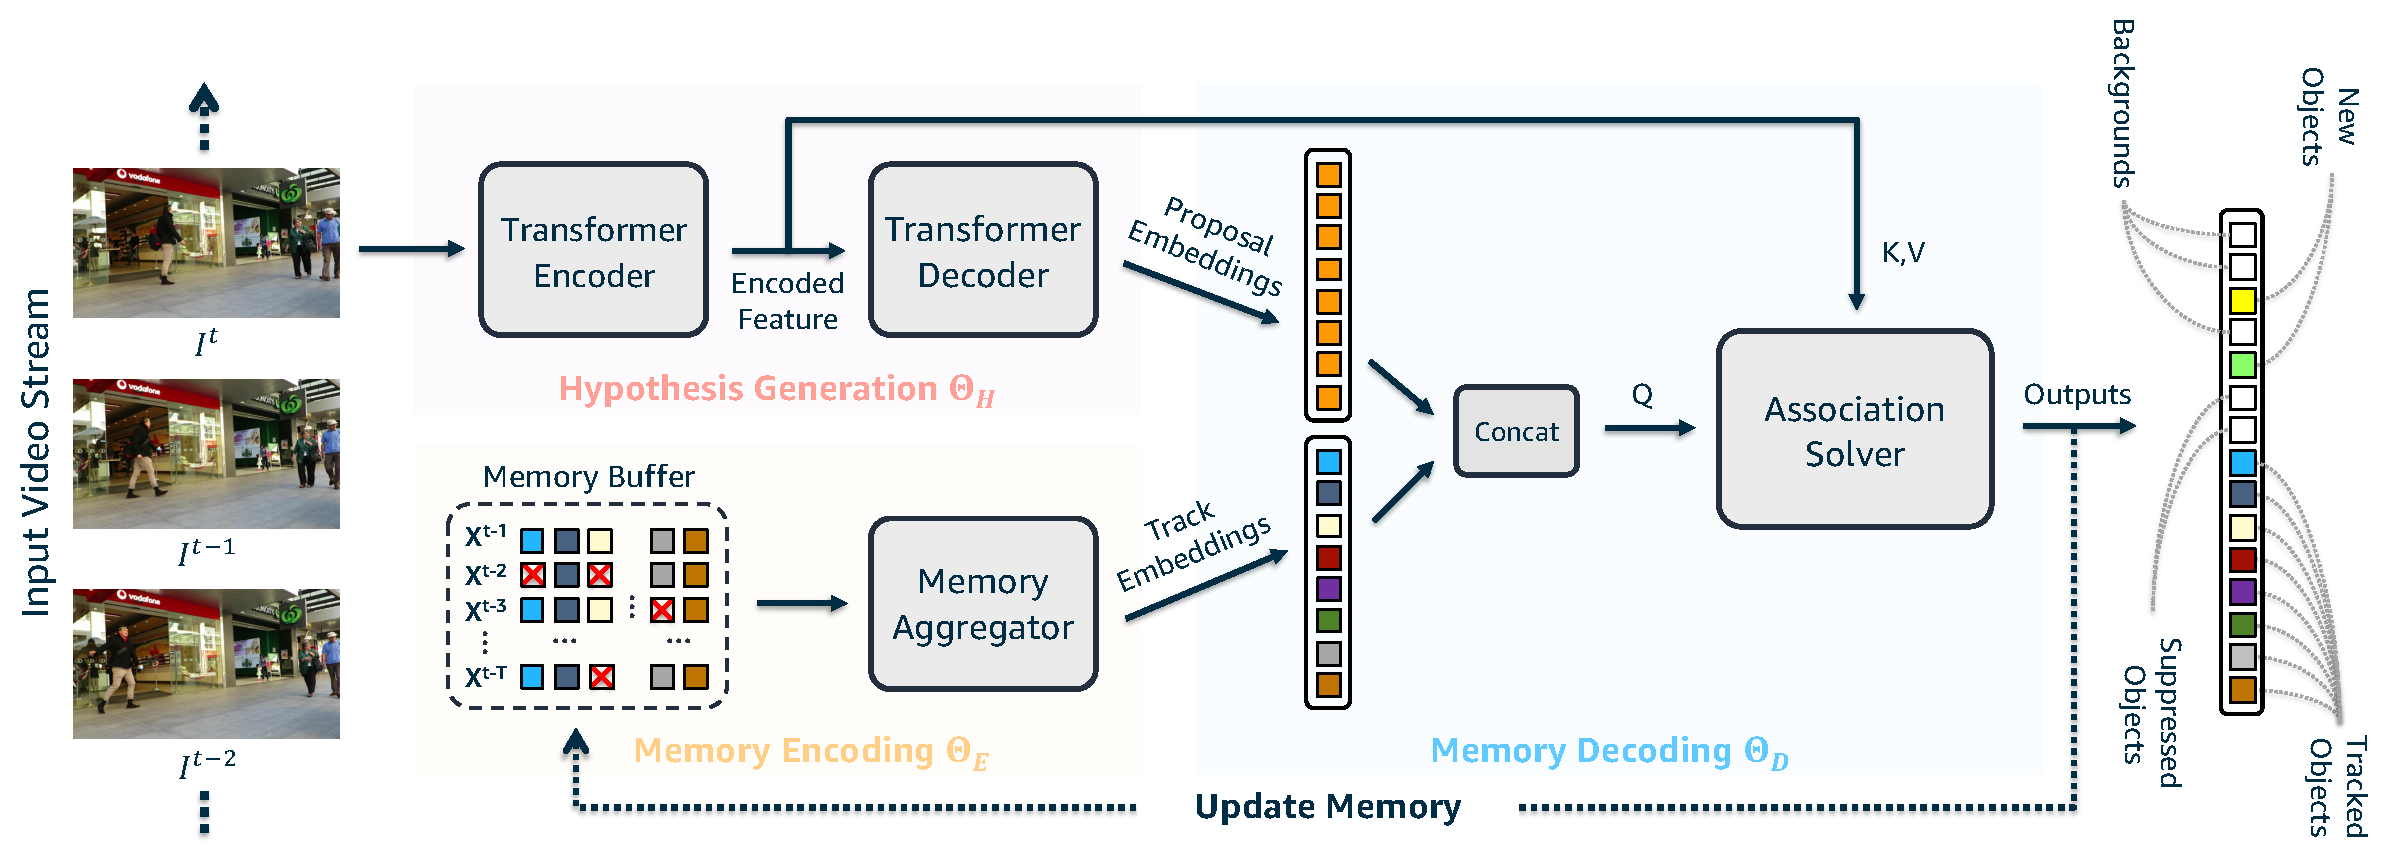
\includegraphics[width=0.97\textwidth]{figures/network.pdf}
    \vspace{-3.5mm}
    \caption{
        \textbf{Visualization of MeMOT}, which runs three main components: 1) a hypothesis generation module $\Theta_H$ that produces object proposals for the current video frame, 2) a memory encoding module $\Theta_E$ that retrieves core information for each tracked objects, and 3) a memory decoding module $\Theta_D$ that solves the object detection and data association tasks simultaneously.
        MeMOT maintains a memory buffer to store long-range states of tracked objects, together with an efficient encoding-decoding process that retrieves useful information for linking objects after a long time span.
        Each hypothetical object is predicted as a new object, a tracked object, or a background region.
    }
    \label{fig:network}
\end{figure*}

\noindent \textbf{Classical Tracking Methods}.
Tracking is well studied in computer vision~\cite{isard1998condensation,babenko2010robust,wu2013online,kristan2015visual}.
Coping with the underlying uncertainties of the tracking results~\cite{isard1998condensation} and object appearances/positions/shapes~\cite{babenko2010robust} has been a central challenge.
Classical non-deep learning methods~\cite{wu2013online} have laid out solid mathematical and statistical foundations.
Specifically, Kalman~\cite{welch1995introduction} and particle filters ~\cite{gustafsson2002particle} are widely adopted for tackling tracking problems~\cite{shen2003probabilistic,hue2001particle,xing2009multi}. The progressive observation-based Bayesian inference method~\cite{xing2010multiple} is proposed for MOT in online sports videos. A spatial and temporal shape representation-based Bayesian framework~\cite{giebel2004bayesian} is proposed for multi-cue 3D deformable object tracking. In these methods,
an optimal filter maintains tracking states that summarize history information and estimate new frame's tracking results. In a linear-Gaussian case, the optimal state can indeed be estimated, while for more general non-linear, non-Gaussian cases, it is difficult to estimate the optimal state with a finite-dimensional state representation. For instance, occlusion in visual multiple object tracking is clearly non-linear and non-Gaussian.
To tackle this challenge, tracking methods~\cite{choi2010multiple,perera2006multi} that can access multiple frames states (offline tracking) is desired.

\vspace{2pt} \noindent \textbf{MOT with CNNs}.
A typical scheme for MOT~\cite{wojke2017simple,feng2019multi,wang2019exploit,chu2019famnet} is ``tracking-by-detection'', which directly uses ready-made detectors~\cite{felzenszwalb2009object,ren2015faster,liu2016ssd,zhou2019objects,ge2021yolox} and focuses on the data association.
% Recent approaches build object detection and data association in the same network.
Tracktor++~\cite{bergmann2019tracking} propagates the bounding boxes of tracked objects as region proposals to the next frame.
CenterTrack~\cite{zhou2020tracking} takes an additional point-based heatmap as input and matches objects anywhere within the receptive field.
JDE~\cite{xu2018joint,wang2019towards,zhang2020fair,li2021semi} is built with two homogeneous branches for object detection and ReID feature extraction, respectively.
Joint detection and tracking models improve the runtime, but sacrifice the tracking recovery after occlusion and cannot reconnect long-term missing objects.

\vspace{2pt} \noindent \textbf{MOT with Transformers}.
Vision Transformers have been successfully applied in image recognition~\cite{carion2020end,dosovitskiy2020image,zhu2020deformable,liu2021swin} and video analysis~\cite{arnab2021vivit,bertasius2021space,sharir2021image,liu2021video} lately.
In tracking, TrackFormer~\cite{meinhardt2021trackformer} and MOTR~\cite{zeng2021motr} simultaneously perform the object detection and association by concatenating the object and autoregressive
track queries as inputs to the Transformer decoder in the next time step.
On the other hand, TransCenter~\cite{xu2021transcenter} and TransTrack~\cite{sun2020transtrack} only use Transformers as feature extractor and recurrently pass track features to aggressively learn aggregated embedding of each object.
TransMOT~\cite{chu2021transmot} still uses CNNs as detector and feature extractor, and learns an affinity matrix with Transformers.
The above work explores the mechanism of representing object states as dynamic embeddings. However, the modeling of long-term spatio-temporal observations and adaptive feature aggregation methods are underdeveloped.

\vspace{3pt} \noindent \textbf{Memory Networks}.
Pioneering work using memory networks has been proposed in NLP~\cite{graves2014neural,weston2014memory,sukhbaatar2015end} by focusing on temporal reasoning tasks such as question answering~\cite{xiong2016dynamic,kumar2016ask} and dialogue systems~\cite{wu2019global}.
Video analysis tasks, such as action recognition~\cite{wu2019long,xu2021long}, and video object segmentation~\cite{oh2019video,lu2020video}, leverage an external memory to store and access time-indexed features in prolonged sequences, significantly improving the ability to remember the past.
Recently, memory networks have been introduced into tracking.
MemTrack~\cite{yang2018learning} reads a residual template from memory and combines it with the initial template to update the representations of targets.
STMTrack~\cite{fu2021stmtrack} guides the information retrieval with the current frame and adaptively obtains all useful information as it needs.
However, these work focuses on single object tracking (SOT), and does not need to concern about the inter-object association.
We propose to use a large spatio-temporal memory to achieve robust object association across time for MOT.
